% Gabarit pandoc des corrigés publiés (brut et guidé). Contenu sans marque ni nom de site.
% Compilation : lualatex (latexmk -lualatex).
% Le Markdown reste la source unique : ne pas éditer ce fichier .tex à la main.
\documentclass[11pt,a4paper]{article}

% --- Moteur, polices (Latin Modern) et langue ---------------------------------
\usepackage{iftex}
\ifLuaTeX\else\errmessage{Ce document se compile avec lualatex}\fi
\usepackage{amsmath,amssymb,mathtools}
\usepackage{fontspec}
% mathrm=sym : \mathrm prend ses glyphes dans la police mathématique (ℓ, μ, Ω), comme KaTeX.
\usepackage[math-style=TeX,bold-style=TeX,mathrm=sym]{unicode-math}
% Repli pour les glyphes absents de Latin Modern (indices et exposants Unicode,
% flèches, filets des schémas en texte, symboles) : DejaVu, puis Latin Modern Math
% (ℓ, lettres mathématiques Unicode des légendes).
\directlua{
  luaotfload.add_fallback("repliTexte", {"DejaVuSerif:mode=harf;", "DejaVuSans:mode=harf;", "file:latinmodern-math.otf:mode=harf;"})
  luaotfload.add_fallback("repliMono", {"DejaVuSansMono:mode=harf;", "DejaVuSans:mode=harf;", "file:latinmodern-math.otf:mode=harf;"})
}
\setmainfont{Latin Modern Roman}[RawFeature={fallback=repliTexte}]
\setsansfont{Latin Modern Sans}[RawFeature={fallback=repliTexte}]
\setmonofont{Latin Modern Mono}[RawFeature={fallback=repliMono}]
\setmathfont{Latin Modern Math}
\usepackage[french]{babel}
\frenchsetup{SmallCapsFigTabCaptions=false}

% --- Mise en page --------------------------------------------------------------
\usepackage[a4paper,margin=2.2cm,headheight=14pt,footskip=1.2cm]{geometry}
\usepackage{microtype}
\setlength{\emergencystretch}{4em}
\tolerance=1500
\setlength{\parindent}{0pt}
\setlength{\parskip}{0.55\baselineskip plus 2pt minus 1pt}
\usepackage{xcolor}
% Gris nommés : babel-french rend « ! » actif dans le document.
\definecolor{gris2}{gray}{0.98}
\definecolor{gris3}{gray}{0.97}
\definecolor{gris5}{gray}{0.95}
\definecolor{gris35}{gray}{0.65}
\definecolor{gris40}{gray}{0.60}
\definecolor{gris45}{gray}{0.55}
\definecolor{gris50}{gray}{0.50}
\definecolor{gris55}{gray}{0.45}
\definecolor{gris60}{gray}{0.40}
\definecolor{gris65}{gray}{0.35}
\definecolor{gris70}{gray}{0.30}
\definecolor{gris80}{gray}{0.20}
\definecolor{gris85}{gray}{0.15}
\usepackage{graphicx}
\usepackage{float}
\usepackage{caption}
\captionsetup{font=small,labelformat=empty,justification=centering}
\usepackage{booktabs,longtable,array,multirow,calc}
\usepackage{siunitx}
\sisetup{locale=FR}
\usepackage[version=4]{mhchem}
\usepackage{listings}
\usepackage{fancyhdr}
\usepackage{lastpage}
\usepackage[most]{tcolorbox}
\usepackage{enumitem}
\setlist{nosep,leftmargin=*,topsep=2pt}
\usepackage[hidelinks,unicode]{hyperref}
\usepackage{bookmark}
\hypersetup{pdftitle={Mines-Ponts PC — Maths 2 2026},pdfauthor={Rédigé par IA},pdfcreator={LaTeX},pdfsubject={Corrigé guidé}}
\usepackage{xurl}

% --- Pandoc : listes, tableaux, figures ----------------------------------------
\providecommand{\passthrough}[1]{#1}
\providecommand{\tightlist}{\setlength{\itemsep}{0pt}\setlength{\parskip}{0pt}}

\makeatletter
\def\maxwidth{\ifdim\Gin@nat@width>\linewidth\linewidth\else\Gin@nat@width\fi}
\def\maxheight{\ifdim\Gin@nat@height>0.55\textheight 0.55\textheight\else\Gin@nat@height\fi}
\makeatother
\setkeys{Gin}{width=\maxwidth,height=\maxheight,keepaspectratio}
\setcounter{secnumdepth}{-\maxdimen}
\providecommand{\pandocbounded}[1]{#1}

% --- Code (listings) -----------------------------------------------------------
\lstset{
  basicstyle=\ttfamily\small,
  columns=fullflexible,
  keepspaces=true,
  breaklines=true,
  breakatwhitespace=false,
  postbreak=\mbox{\textcolor{gris50}{$\hookrightarrow$}\space},
  frame=single,
  rulecolor=\color{gris35},
  framesep=4pt,
  xleftmargin=5pt,xrightmargin=5pt,
  backgroundcolor=\color{gris3},
  keywordstyle=\bfseries,
  commentstyle=\color{gris65},
  stringstyle=\color{gris80},
  showstringspaces=false,
  tabsize=4,
  extendedchars=true,
  aboveskip=6pt,belowskip=6pt,
}

% --- Macros des corrigés (KaTeX ↔ LaTeX) ---------------------------------------
% Les corrigés sont écrits pour KaTeX : on définit ici ce que KaTeX connaît et
% que LaTeX n'a pas, sans jamais retoucher le Markdown.
\providecommand{\R}{\mathbb{R}}
\providecommand{\N}{\mathbb{N}}
\providecommand{\Z}{\mathbb{Z}}
\providecommand{\Q}{\mathbb{Q}}
\providecommand{\C}{\mathbb{C}}
\providecommand{\dd}{\mathrm{d}}
\providecommand{\llbracket}{\lBrack}
\providecommand{\rrbracket}{\rBrack}
\providecommand{\lBrace}{\lbrace}
\providecommand{\rBrace}{\rbrace}
\providecommand{\Box}{\square}
\providecommand{\Diamond}{\lozenge}
\providecommand{\varnothing}{\emptyset}
\providecommand{\argmax}{\operatorname*{arg\,max}}
\providecommand{\argmin}{\operatorname*{arg\,min}}
\renewcommand{\leq}{\leqslant}
\renewcommand{\geq}{\geqslant}

% Équation hors texte : réduite à la largeur de la ligne si elle déborde.
\newsavebox{\boiteequation}
\newcommand{\equationajustee}[1]{%
  \sbox{\boiteequation}{$\displaystyle #1$}%
  \ifdim\wd\boiteequation>\linewidth
    \[\resizebox{\linewidth}{!}{\usebox{\boiteequation}}\]%
  \else
    \[#1\]%
  \fi}

% --- Encadrés pédagogiques (sobres, lisibles en noir et blanc) -----------------
\tcbset{
  encadre/.style={
    enhanced,breakable,sharp corners,
    colback=white,colframe=gris55,
    boxrule=0.4pt,leftrule=2.2pt,
    left=6pt,right=6pt,top=3pt,bottom=3pt,
    before skip=6pt,after skip=6pt,
    fonttitle=\bfseries\small,coltitle=black,
    attach title to upper,after title={\quad},
    parbox=false,
  }
}
\newtcolorbox{indication}[1]{encadre,colframe=gris45,colback=gris2,title={Indication~#1}}
\newtcolorbox{methode}{encadre,colframe=gris70,title={Méthode}}
\newtcolorbox{piege}{encadre,colframe=gris85,boxrule=0.8pt,leftrule=2.2pt,title={Piège}}
\newtcolorbox{jury}{encadre,colframe=gris60,colback=gris5,title={Jury}}
\newtcolorbox{encadrenote}{encadre,colframe=gris40}

% --- Titres de section ---------------------------------------------------------
\usepackage{titlesec}
\titleformat{\section}{\Large\bfseries}{}{0pt}{}
\titleformat{\subsection}{\large\bfseries}{}{0pt}{}
\titleformat{\subsubsection}{\normalsize\bfseries}{}{0pt}{}
\titlespacing*{\section}{0pt}{14pt plus 4pt minus 2pt}{6pt}
\titlespacing*{\subsection}{0pt}{10pt plus 3pt minus 2pt}{4pt}
\titlespacing*{\subsubsection}{0pt}{8pt plus 2pt minus 2pt}{2pt}

% --- En-tête et pied de page ---------------------------------------------------
\pagestyle{fancy}
\fancyhf{}
\fancyhead[L]{\small\textsc{Corrigé guidé} · Mines-Ponts PC}
\fancyhead[R]{\small Maths 2 2026}
\fancyfoot[L]{\footnotesize Corrigé rédigé par IA, non officiel}
\fancyfoot[R]{\footnotesize \thepage\,/\,\pageref*{LastPage}}
\renewcommand{\headrulewidth}{0.4pt}
\renewcommand{\footrulewidth}{0pt}
\fancypagestyle{plain}{\fancyhf{}\fancyfoot[R]{\footnotesize \thepage\,/\,\pageref*{LastPage}}\fancyfoot[L]{\footnotesize Corrigé rédigé par IA, non officiel}\renewcommand{\headrulewidth}{0pt}}

\begin{document}
\thispagestyle{plain}
\begin{center}
  {\small\scshape Corrigé guidé}\par\smallskip
  {\LARGE\bfseries Mines-Ponts PC — Maths 2 2026\par}\medskip
  {\large Mines-Ponts · PC · Maths 2 · 2026\par}
\end{center}
\vspace{2pt}\hrule\vspace{8pt}

\emph{Corrigé rédigé par IA, non officiel. Signalez toute erreur.}

\hypertarget{pruxe9sentation-du-sujet}{%
\section{Présentation du sujet}\label{pruxe9sentation-du-sujet}}

\textbf{Thème.} Le problème étudie l'équation différentielle linéaire du second ordre
\equationajustee{(E)\quad y''+b(x)y=c(x),}
où \(b\) et \(c\) sont continues et \(2\pi\)-périodiques. Il pose une seule question sous plusieurs angles : quand \((E)\) possède-t-elle une solution périodique ?

Le fil conducteur est le critère de la question 4 : une solution qui « recolle » en valeur \textbf{et} en dérivée entre \(0\) et \(2\pi\) est \(2\pi\)-périodique. Chaque partie fabrique, par un moyen différent, une solution qui recolle.

\textbf{Découpage (25 questions, 3 heures, sans calculatrice ni document).}

\begin{itemize}
\tightlist
\item
  \textbf{Partie 1 (Q1--Q4), résultats généraux} : structure des solutions bornées, opérateur de translation \(T\), critère de périodicité. Courte et réutilisée partout.
\item
  \textbf{Partie 2 (Q5--Q10), coefficients constants} : \(y''+\omega^2y=\cos x\). Calcul explicite ; l'existence de solutions périodiques autres que \(f_0\) dépend de la rationalité de \(\omega\).
\item
  \textbf{Partie 3 (Q11--Q14), \(b=-(1+\cos x)\)} : un argument de convexité donne l'unicité de la solution bornée, puis sa périodicité.
\item
  \textbf{Partie 4 (Q15--Q21), toujours \(b=-(1+\cos x)\)} : construction d'une solution périodique quand \(c\) est une combinaison finie de \(\sin(nx)\), par une série de sinus et un argument d'algèbre linéaire « en degré ».
\item
  \textbf{Partie 5 (Q22--Q25), théorème général} : si une solution \(f_0\) est bornée ainsi que sa dérivée, il existe une solution périodique. Argument de compacité en dimension finie et de moyennes de translatées.
\end{itemize}

\textbf{Notions mobilisées.} Principe de superposition ; équations à coefficients constants ; périodicité ; convexité via la dérivée seconde ; séries numériques (comparaison, Riemann) ; séries de fonctions (convergence normale, dérivation terme à terme de classe \(\mathcal C^2\)) ; linéarisation trigonométrique ; familles libres, bases, dimension, somme directe ; topologie en dimension finie (continuité des applications linéaires, caractérisation séquentielle des fermés, théorème des bornes atteintes).

\textbf{Ce qu'en dit le rapport 2026.} Le jury juge les questions « pour la plupart très simples et le sujet raisonnablement court », et regrette que son attente ait été souvent déçue. Hors les 20 \% de copies les plus faibles, la plupart des candidats ont abordé les 21 premières questions ; les notes ont reflété la précision des arguments, notamment le recours au cours.

\textbf{Question neutralisée.} Le théorème de Cauchy n'est pas au programme de PC pour les équations d'ordre 2 à coefficients non constants, et le jury a neutralisé la question 4. Ce corrigé démontre directement, par une méthode d'énergie, l'unicité dont Q4 et Q25 ont besoin.

\textbf{Difficulté et gestion du temps.} Sujet de longueur raisonnable, sans calcul lourd, très progressif. Les parties 2, 3 et 4 sont indépendantes entre elles ; la partie 5 n'utilise que la partie 1.

Questions à ne pas laisser passer : Q1 à Q3, Q5, Q6, Q8, Q10, Q13, Q17, Q18, Q21, Q25 (rédigeable en admettant Q23 et Q24).

Questions discriminantes selon le rapport 2026 : Q1 et Q2 (le caractère borné, très souvent oublié ; les deux inclusions), Q11 (dérivée seconde de \(g^2\)), Q12 (de \(g^2\) constante à \(g\) nulle), Q14 (« Très peu traité correctement »), Q15 (la série \(\sum n^2a_n\)), Q16 (dérivation terme à terme), Q19--Q20 (inclusions \(L(\mathcal P)\subset\mathcal P\) et \(L(\mathcal P_N)\subset\mathcal P_{N+1}\)), puis toute la partie 5, « partie peu abordée, du moins correctement ».

\textbf{Convexité.} La caractérisation des fonctions convexes de classe \(\mathcal C^2\) par le signe de la dérivée seconde est vue en terminale, et le rapport 2026 la compte parmi les outils attendus en Q11. On la redémontre brièvement en Q11 ; le résultat clé (une fonction convexe non constante n'est pas majorée) est admis par l'énoncé.

\hypertarget{partie-1-ruxe9sultats-guxe9nuxe9raux}{%
\section{Partie 1 --- Résultats généraux}\label{partie-1-ruxe9sultats-guxe9nuxe9raux}}

Tout repose sur la \textbf{linéarité} de \(y\mapsto y''+by\) (principe de superposition) et sur un \textbf{lemme d'unicité}, démontré en Q4 sans le théorème de Cauchy : une solution de \((EH)\) nulle en \(0\) ainsi que sa dérivée est la fonction nulle.

\hypertarget{question-1}{%
\subsection{Question 1}\label{question-1}}

\begin{indication}{1}

Montrer qu'une partie est un sous-espace vectoriel d'un espace vectoriel connu : inclusion, non-vacuité, stabilité par combinaison linéaire.

\end{indication}

\begin{indication}{2}

La seule chose à vérifier vraiment, c'est que la combinaison linéaire reste bornée : écrire une majoration indépendante de \(x\).

\end{indication}

\hypertarget{solution}{%
\subsubsection{Solution}\label{solution}}

On a \(\mathcal B(H)=\mathcal S(H)\cap\mathbf B(\mathbb R,\allowbreak \mathbb R)\subset\mathcal S(H)\). La fonction nulle est une solution bornée de \((EH)\).

Soient \(g_1,g_2\in\mathcal B(H)\) et \(\lambda\in\mathbb R\). On a \(\lambda g_1+g_2\in\mathcal S(H)\) car \(\mathcal S(H)\) est un espace vectoriel, et pour tout \(x\),
\equationajustee{|\lambda g_1(x)+g_2(x)|\le|\lambda|\,\|g_1\|+\|g_2\|,}
majorant indépendant de \(x\). Donc \(\lambda g_1+g_2\in\mathcal B(H)\).

\textbf{\(\mathcal B(H)\) est un sous-espace vectoriel de \(\mathcal S(H)\).}

\begin{methode}

L'intersection de deux sous-espaces vectoriels d'un même espace est un sous-espace : ici \(\mathcal S(H)\) et \(\mathbf B(\mathbb R,\mathbb R)\) sont deux sous-espaces de l'espace des fonctions de \(\mathbb R\) dans \(\mathbb R\). C'est une rédaction encore plus courte.

\end{methode}

\begin{jury}

Rapport 2026 : « De très nombreux candidats ne se sont pas du tout intéressés au caractère borné ». Ils se sont contentés de montrer que \(\mathcal S(H)\) est un espace vectoriel, propriété du cours qu'il n'y avait pas à redémontrer. Tout l'enjeu est la majoration.

\end{jury}

\hypertarget{question-2}{%
\subsection{Question 2}\label{question-2}}

\begin{indication}{1}

Égalité d'ensembles : double inclusion.

\end{indication}

\begin{indication}{2}

La différence de deux solutions de \((E)\) est solution de \((EH)\), et la somme d'une solution de \((E)\) et d'une solution de \((EH)\) est solution de \((E)\). N'oublier dans aucun sens le caractère borné.

\end{indication}

\hypertarget{solution-1}{%
\subsubsection{Solution}\label{solution-1}}

Soit \(f_0\in\mathcal B(E)\).

\begin{itemize}
\item
  Soit \(f\in\mathcal B(E)\) et \(g=f-f_0\). Cette fonction est de classe \(\mathcal C^2\) et vérifie \(g''+bg=c-c=0\) : elle est solution de \((EH)\).

  Elle est bornée, par \(\|f\|+\|f_0\|\). Donc \(g\in\mathcal B(H)\), et \(f\) s'écrit \(f_0+g\).
\item
  Si \(g\in\mathcal B(H)\), alors \(f_0+g\) est de classe \(\mathcal C^2\) et \((f_0+g)''+b(f_0+g)=c\). Elle est bornée comme somme de fonctions bornées. Donc \(f_0+g\in\mathcal B(E)\).
\end{itemize}

\equationajustee{\boxed{\mathcal B(E)=\{f_0+g,\ g\in\mathcal B(H)\}.}}

\begin{piege}

La consigne de l'énoncé, vérifier que les éléments de \(\mathcal B(E)\) sont les fonctions de la forme \(f_0+g\), demande les \textbf{deux} inclusions, pas seulement que tout élément de \(\mathcal B(E)\) s'écrit ainsi. Et dans chaque sens, il y a deux propriétés à vérifier : être solution, et être bornée.

\end{piege}

\begin{jury}

Rapport 2026 : la formulation a été mal interprétée, les candidats croyant presque tous qu'un seul sens d'implication était demandé, « alors qu'il s'agissait de montrer une égalité entre deux ensembles ». Le caractère borné y a été négligé comme en Q1.

\end{jury}

\hypertarget{question-3}{%
\subsection{Question 3}\label{question-3}}

\begin{indication}{1}

Calculer \(T(f)''(x)\) en fonction de \(f''\), puis appliquer l'équation au point \(x+2\pi\).

\end{indication}

\begin{indication}{2}

Repérer précisément où servent la périodicité de \(b\) et celle de \(c\).

\end{indication}

\hypertarget{solution-2}{%
\subsubsection{Solution}\label{solution-2}}

Soit \(f\in\mathcal S(E)\). La fonction \(T(f)\) est la composée de \(f\) avec la translation \(x\mapsto x+2\pi\), donc de classe \(\mathcal C^2\), et \(T(f)''(x)=f''(x+2\pi)\).

Pour tout \(x\), comme \(b(x)=b(x+2\pi)\) puis \(c(x+2\pi)=c(x)\) :
\equationajustee{\begin{aligned}
T(f)''(x)+b(x)T(f)(x)&=f''(x+2\pi)+b(x+2\pi)f(x+2\pi)\\
&=c(x+2\pi)\\
&=c(x).
\end{aligned}}
\textbf{\(T(f)\) est solution de \((E)\).}

Deux remarques utiles pour la suite. Avec \(c=0\), \(T\) envoie \(\mathcal S(H)\) dans lui-même.

Et si \(f\) est bornée, \(\|T(f)\|=\|f\|\), car \(x\mapsto x+2\pi\) est une bijection de \(\mathbb R\) :
\equationajustee{\sup_{x\in\mathbb R}|f(x+2\pi)|=\sup_{t\in\mathbb R}|f(t)|.}

\hypertarget{question-4}{%
\subsection{Question 4}\label{question-4}}

\begin{indication}{1}

Suivre l'indication : de quelle équation \(h=T(f)-f\) est-elle solution ? Que valent \(h(0)\) et \(h'(0)\) ?

\end{indication}

\begin{indication}{2}

Le théorème de Cauchy pour l'ordre 2 à coefficients non constants n'est pas au programme de PC. Pour montrer \(h=0\), étudier l'« énergie » \(E=h^2+h'^2\) : majorer \(|E'|\) par un multiple de \(E\).

\end{indication}

\begin{indication}{3}

Une fonction positive, nulle en \(0\), telle que \(x\mapsto e^{-Kx}E(x)\) décroît sur \([0,+\infty[\), est nulle sur cet intervalle.

\end{indication}

\hypertarget{solution-3}{%
\subsubsection{Solution}\label{solution-3}}

Posons \(h=T(f)-f\). Par la question 3, \(T(f)\in\mathcal S(E)\), et \(f\in\mathcal S(E)\) ; par superposition, \(h\in\mathcal S(H)\). De plus
\equationajustee{\begin{aligned}
h(0)&=f(2\pi)-f(0)\\
&=0,\\[1mm]
h'(0)&=f'(2\pi)-f'(0)\\
&=0.
\end{aligned}}

\emph{Lemme d'unicité : une solution \(h\) de \((EH)\) telle que \(h(0)=h'(0)=0\) est nulle.}

La fonction \(b\) est continue et \(2\pi\)-périodique, donc bornée (résultat admis par l'énoncé).

On pose \(K=1+\|b\|\) et \(E=h^2+h'^2\), de classe \(\mathcal C^1\), positive, nulle en \(0\). Avec \(h''=-bh\) :
\equationajustee{\begin{aligned}
E'&=2hh'+2h'h''\\
&=2(1-b)hh'.
\end{aligned}}
Comme \(2|hh'|\le h^2+h'^2\), on obtient \(|E'|\le KE\) sur \(\mathbb R\).

\begin{itemize}
\tightlist
\item
  Sur \([0,+\infty[\), la dérivée de \(x\mapsto e^{-Kx}E(x)\) est \(e^{-Kx}(E'-KE)\le0\). Cette fonction est décroissante, positive et nulle en \(0\) : elle est nulle.
\item
  Sur \(]-\infty,0]\), la dérivée de \(x\mapsto e^{Kx}E(x)\) est \(e^{Kx}(E'+KE)\ge0\). Cette fonction est croissante, positive et nulle en \(0\) : elle est nulle.
\end{itemize}

Donc \(E=0\), puis \(h=0\) : pour tout \(x\in\mathbb R\), \(f(x+2\pi)=f(x)\).

\textbf{\(f\) est \(2\pi\)-périodique.}

Le lemme a une autre conséquence, utile en partie 5. L'application \(g\mapsto(g(0),g'(0))\) est linéaire de \(\mathcal S(H)\) dans \(\mathbb R^2\) et injective, donc \(\dim\mathcal S(H)\le2\).

\begin{methode}

Pour montrer que deux solutions d'une équation linéaire coïncident, on montre que leur différence est solution de l'équation homogène avec des conditions initiales nulles, puis on prouve l'unicité. Sans le théorème de Cauchy, la méthode d'énergie (majorer \(|E'|\) par \(KE\), puis étudier \(e^{\mp Kx}E\)) suffit. C'est le réflexe central du sujet : il resservira en Q25.

\end{methode}

\begin{piege}

« \(h(0)=h'(0)=0\) donc \(h=0\) » n'est pas un argument : une fonction quelconque peut s'annuler avec sa dérivée en un point sans être nulle. C'est l'équation différentielle qui rend la conclusion vraie, et il faut un théorème ou une preuve pour l'exploiter.

\end{piege}

\begin{jury}

Rapport 2026 : « Le théorème de Cauchy n'est pas au programme de PCSI-PC dans le contexte des équations différentielles d'ordre 2 à coefficients non constants. » Seuls de rares candidats l'ont invoqué, et « Au final le jury a décidé de neutraliser cette question pour ne pas introduire d'inéquité. »

\end{jury}

\hypertarget{partie-2-un-exemple-duxe9quation-uxe0-coefficients-constants}{%
\section{Partie 2 --- Un exemple d'équation à coefficients constants}\label{partie-2-un-exemple-duxe9quation-uxe0-coefficients-constants}}

On résout explicitement \(y''+\omega^2y=\cos x\) (\(\omega>0\), \(\omega\neq1\)), puis on cherche ses solutions périodiques. Outils : équations à coefficients constants, déterminant \(2\times2\), arithmétique élémentaire sur les rationnels.

\hypertarget{question-5}{%
\subsection{Question 5}\label{question-5}}

\begin{indication}{1}

Reporter \(f_0=d\cos\) dans l'équation et identifier ; à quoi sert l'hypothèse \(\omega\neq1\) ?

\end{indication}

\begin{indication}{2}

Pour \(u\) et \(v\) : écrire la solution générale réelle de \(y''+\omega^2y=0\) et ajuster les deux constantes aux conditions initiales.

\end{indication}

\hypertarget{solution-4}{%
\subsubsection{Solution}\label{solution-4}}

Pour \(f_0(x)=d\cos x\), on a \(f_0''+\omega^2f_0=d(\omega^2-1)\cos\). Cette fonction est égale à \(\cos\) si et seulement si \(d(\omega^2-1)=1\) (évaluer en \(0\) pour le sens direct).

Comme \(\omega>0\) et \(\omega\neq1\), on a \(\omega^2\neq1\) et
\equationajustee{\boxed{d=\frac{1}{\omega^2-1}.}}
L'équation caractéristique \(r^2+\omega^2=0\) a pour racines \(\pm i\omega\).

Les solutions réelles de \((EH)\) sont les \(x\mapsto\alpha\cos(\omega x)+\beta\sin(\omega x)\), de valeur \(\alpha\) et de dérivée \(\beta\omega\) en \(0\). Les conditions imposées donnent
\equationajustee{\boxed{u(x)=\cos(\omega x)}}
\equationajustee{\boxed{v(x)=\frac{\sin(\omega x)}{\omega}.}}

\begin{piege}

Le facteur \(1/\omega\) dans \(v\) est imposé par \(v'(0)=1\) ; il se retrouve dans le système de la question 8. Pour \(\omega=1\) (résonance), aucune solution de la forme \(d\cos\) n'existe : c'est pourquoi l'énoncé l'exclut.

\end{piege}

\begin{jury}

Rapport 2026 : les erreurs de calcul, plutôt rares, ont été sanctionnées, car « on attend des candidats la capacité à mener un calcul juste jusqu'à son terme ». Vérifier \(u(0)\), \(u'(0)\), \(v(0)\), \(v'(0)\) avant de passer à la suite.

\end{jury}

\hypertarget{question-6}{%
\subsection{Question 6}\label{question-6}}

\begin{indication}{1}

Structure de l'ensemble des solutions d'une équation linéaire : solution particulière plus solutions de l'équation homogène.

\end{indication}

\begin{indication}{2}

Pour \(\mathcal B(E)\), se demander si toutes les solutions trouvées sont bornées.

\end{indication}

\hypertarget{solution-5}{%
\subsubsection{Solution}\label{solution-5}}

Par superposition, \(\mathcal S(E)=f_0+\mathcal S(H)\), et \(\mathcal S(H)=\operatorname{Vect}(u,v)\) (cours sur les équations à coefficients constants) :
\equationajustee{\boxed{\mathcal S(E)=\Big\{x\mapsto\frac{\cos x}{\omega^2-1}+A\cos(\omega x)+\frac B\omega\sin(\omega x),\ (A,B)\in\mathbb R^2\Big\}.}}
Pour une telle \(f\) et tout \(x\), \(|f(x)|\le\frac{1}{|\omega^2-1|}+|A|+\frac{|B|}{\omega}\) : toute solution est bornée. Donc
\equationajustee{\boxed{\mathcal B(E)=\mathcal S(E).}}

\begin{piege}

L'égalité \(\mathcal B(E)=\mathcal S(E)\) est propre à cet exemple (\(b=\omega^2>0\) donne des oscillations bornées). En partie 3 au contraire, \(\mathcal B(E)\) a au plus un élément.

\end{piege}

\hypertarget{question-7}{%
\subsection{Question 7}\label{question-7}}

\begin{indication}{1}

Plutôt que de discuter les périodes de \(\cos x\), \(\cos(\omega x)\), \(\sin(\omega x)\) séparément, faire agir la périodicité de \(f\) sur l'équation elle-même.

\end{indication}

\begin{indication}{2}

Si \(f\) est \(T\)-périodique, \(f''\) l'est aussi ; que dire alors du second membre ?

\end{indication}

\hypertarget{solution-6}{%
\subsubsection{Solution}\label{solution-6}}

Soit \(T>0\) une période de \(f\). On dérive deux fois \(f(x+T)=f(x)\), ce qui est licite car \(f\) est de classe \(\mathcal C^2\).

On obtient \(f''(x+T)=f''(x)\). Donc, pour tout \(x\),
\equationajustee{\begin{aligned}
\cos(x+T)&=f''(x+T)+\omega^2f(x+T)\\
&=f''(x)+\omega^2f(x)\\
&=\cos x.
\end{aligned}}
En \(x=0\) : \(\cos T=1\), donc \(T\in2\pi\mathbb Z\), et comme \(T>0\) :
\equationajustee{\boxed{T=2k\pi,\quad k\in\mathbb N^*.}}

\begin{piege}

Raisonner à l'envers : partir des périodes de \(\cos\) et de \(\cos(\omega\,\cdot)\) pour en déduire celle de \(f\). Seule la combinaison \(f\) est supposée périodique, et rien ne dit a priori que \(T\) soit une période de chacun des termes.

\end{piege}

\begin{jury}

Rapport 2026 : « Il fallait partir de la périodicité de \(f\) pour arriver à celle de cos et non le contraire comme trop souvent observé. »

\end{jury}

\hypertarget{question-8}{%
\subsection{Question 8}\label{question-8}}

\begin{indication}{1}

Une fonction \(T\)-périodique dérivable a une dérivée \(T\)-périodique : écrire \(f(2k\pi)=f(0)\) et \(f'(2k\pi)=f'(0)\).

\end{indication}

\begin{indication}{2}

Expliciter \(f\) et sa dérivée à l'aide de \(u\), \(v\) et \(f_0\). Les valeurs du cosinus et du sinus en \(2k\pi\) font disparaître \(f_0\) des différences.

\end{indication}

\hypertarget{solution-7}{%
\subsubsection{Solution}\label{solution-7}}

Posons \(\theta=2k\pi\omega\). On a
\equationajustee{\begin{aligned}
f(x)&=d\cos x+A\cos(\omega x)+\frac B\omega\sin(\omega x),\\
f'(x)&=-d\sin x-A\omega\sin(\omega x)+B\cos(\omega x).
\end{aligned}}
Comme \(k\) est entier,
\equationajustee{\begin{aligned}
f(0)&=d+A,\\
f(2k\pi)&=d+A\cos\theta+\frac B\omega\sin\theta,\\
f'(0)&=B,\\
f'(2k\pi)&=-A\omega\sin\theta+B\cos\theta.
\end{aligned}}
Par la question 7, \(f\) est \(2k\pi\)-périodique, donc \(f'\) aussi : \(f(2k\pi)=f(0)\) et \(f'(2k\pi)=f'(0)\). En soustrayant :
\equationajustee{\boxed{\begin{cases}(\cos(2k\pi\omega)-1)A+\dfrac{\sin(2k\pi\omega)}{\omega}B=0\\[2mm]-\omega\sin(2k\pi\omega)A+(\cos(2k\pi\omega)-1)B=0.\end{cases}}}

\begin{methode}

Les deux conditions \(f(T)=f(0)\) et \(f'(T)=f'(0)\) sont exactement celles du critère de la question 4 (avec \(2k\pi\) au lieu de \(2\pi\)) : pour une équation du second ordre, deux conditions de recollement suffisent.

\end{methode}

\hypertarget{question-9}{%
\subsection{Question 9}\label{question-9}}

\begin{indication}{1}

Calculer \(\det M\) en fonction de \(\theta=2k\pi\omega\) ; le résultat se simplifie grâce à \(\cos^2+\sin^2=1\).

\end{indication}

\begin{indication}{2}

Quand ce déterminant s'annule-t-il ? Utiliser ensuite l'irrationalité de \(\omega\) avec \(k\) entier non nul, puis le théorème sur les systèmes de Cramer.

\end{indication}

\hypertarget{solution-8}{%
\subsubsection{Solution}\label{solution-8}}

\equationajustee{\begin{aligned}
\det M&=(\cos\theta-1)^2-\frac{\sin\theta}{\omega}\cdot(-\omega\sin\theta)\\
&=(\cos\theta-1)^2+\sin^2\theta\\
&=2(1-\cos\theta)\\
&=4\sin^2(k\pi\omega).
\end{aligned}}
Il est nul si et seulement si \(\cos\theta=1\), c'est-à-dire \(\theta\in2\pi\mathbb Z\), c'est-à-dire \(k\omega\in\mathbb Z\).

Supposons \(\omega\notin\mathbb Q\), et soit \(f\) une solution périodique, de période \(2k\pi\) avec \(k\in\mathbb N^*\) (question 7). Si l'on avait \(k\omega=m\in\mathbb Z\), alors \(\omega=m/k\) serait rationnel : exclu.

Donc \(\det M\neq0\) : la matrice \(M\) est inversible, et le système homogène de la question 8, de Cramer, n'a que la solution nulle. Ainsi \(A=B=0\) et \(f=f_0\).

Réciproquement, \(f_0=d\cos\) est bien une solution \(2\pi\)-périodique.

\textbf{Si \(\omega\notin\mathbb Q\), la seule solution périodique de \((E)\) est \(f_0\).}

\begin{piege}

Le sens à retenir : déterminant \textbf{non nul}, donc système de Cramer, donc solution unique, ici la solution nulle d'un système homogène. Un déterminant nul ne donnerait pas l'unicité. Ne pas oublier non plus la réciproque : \(f_0\) \textbf{est} une solution périodique.

\end{piege}

\begin{jury}

Rapport 2026 : question d'algèbre linéaire élémentaire qui a causé des écarts, « certains se mélangeant entre déterminant nul ou non nul et son application aux systèmes de Cramer ». L'irrationalité de \(\omega\) a aussi été mal exploitée dans la rédaction : écrire explicitement que \(k\omega\in\mathbb Z\) forcerait \(\omega=m/k\in\mathbb Q\).

\end{jury}

\hypertarget{question-10}{%
\subsection{Question 10}\label{question-10}}

\begin{indication}{1}

Chercher un réel qui soit à la fois multiple de \(2\pi\) (période de \(\cos\)) et multiple de \(2\pi/\omega\) (période de \(\cos(\omega x)\) et \(\sin(\omega x)\)).

\end{indication}

\begin{indication}{2}

Une seule période commune suffit : proposer un candidat simple en fonction de \(q\) et le vérifier.

\end{indication}

\hypertarget{solution-9}{%
\subsubsection{Solution}\label{solution-9}}

Soit \(\omega=p/q\) avec \(p,q\in\mathbb N^*\), et \(f\in\mathcal S(E)\) quelconque :
\equationajustee{f(x)=d\cos x+A\cos(\omega x)+\frac B\omega\sin(\omega x).}
Comme \(2q\pi\in2\pi\mathbb Z\), on a \(\cos(x+2q\pi)=\cos x\). Et \(\omega(x+2q\pi)=\omega x+2p\pi\).

Donc \(\cos(\omega(x+2q\pi))=\cos(\omega x)\) et \(\sin(\omega(x+2q\pi))=\sin(\omega x)\). Ainsi \(f(x+2q\pi)=f(x)\) pour tout \(x\) :
\equationajustee{\boxed{2q\pi\ \text{est une \text{période} commune \text{à} toutes les solutions de }(E).}}

\begin{methode}

La question demande \textbf{une} période commune, pas la plus petite : inutile de supposer la fraction irréductible ou de discuter des parités. C'est cohérent avec Q9 : pour \(k=q\), \(k\omega=p\in\mathbb Z\) et \(\det M=0\).

\end{methode}

\begin{jury}

Rapport 2026 : « Le sujet ne demandait pas la période optimale, ce que les candidats ont bien compris. »

\end{jury}

\hypertarget{partie-3-unicituxe9-lorsque-la-fonction-b-est-nuxe9gative}{%
\section{\texorpdfstring{Partie 3 --- Unicité lorsque la fonction \(b\) est négative}{Partie 3 --- Unicité lorsque la fonction b est négative}}\label{partie-3-unicituxe9-lorsque-la-fonction-b-est-nuxe9gative}}

Avec \(b=-(1+\cos x)\le0\), l'équation homogène \(y''=(1+\cos x)y\) n'admet pas d'oscillation : une solution non nulle « s'emballe ». La convexité de \(g^2\) traduit ce fait et donne l'unicité de la solution bornée, puis sa périodicité grâce à \(T\).

\hypertarget{question-11}{%
\subsection{Question 11}\label{question-11}}

\begin{indication}{1}

Calculer \((g^2)''\) pas à pas (dériver \(g^2\), puis dériver le résultat), et remplacer \(g''\) à l'aide de l'équation.

\end{indication}

\begin{indication}{2}

Pour conclure, utiliser la caractérisation de la convexité des fonctions de classe \(\mathcal C^2\) par le signe de la dérivée seconde.

\end{indication}

\hypertarget{solution-10}{%
\subsubsection{Solution}\label{solution-10}}

\emph{Critère (rappel).} Soit \(\varphi\in\mathcal C^2(\mathbb R,\mathbb R)\) avec \(\varphi''\ge0\) ; alors \(\varphi'\) est croissante.

Soient \(x<y\), \(\lambda\in\,]0,1[\) et \(z=\lambda x+(1-\lambda)y\), de sorte que \(z-x=(1-\lambda)(y-x)\) et \(y-z=\lambda(y-x)\).

L'égalité des accroissements finis fournit \(c_1\in\,]x,z[\) et \(c_2\in\,]z,y[\) tels que :
\equationajustee{\begin{aligned}
\varphi(z)-\varphi(x)&=\varphi'(c_1)(z-x),\\
\varphi(y)-\varphi(z)&=\varphi'(c_2)(y-z).
\end{aligned}}
Alors
\equationajustee{\begin{aligned}
\lambda\varphi(x)+(1-\lambda)\varphi(y)-\varphi(z)&=-\lambda(\varphi(z)-\varphi(x))+(1-\lambda)(\varphi(y)-\varphi(z))\\
&=\lambda(1-\lambda)(y-x)\big(\varphi'(c_2)-\varphi'(c_1)\big)\\
&\ge0.
\end{aligned}}
Les cas \(\lambda\in\{0,1\}\) ou \(x=y\) sont immédiats : \(\varphi\) est convexe.

\emph{Application.} Soit \(g\in\mathcal S(H)\) et \(\varphi=g^2\), de classe \(\mathcal C^2\). Alors \(\varphi'=2gg'\) et
\equationajustee{\begin{aligned}
\varphi''&=2g'^2+2gg''\\
&=2g'^2+2(1+\cos x)g^2.
\end{aligned}}
Les deux termes sont positifs car \(1+\cos x\ge0\) pour tout réel \(x\). Donc \(\varphi''\ge0\) et \textbf{\(g^2\) est convexe.}

\begin{piege}

Deux erreurs relevées par le jury. Écrire \((g^2)''=2gg''\) ou \((g'')^2\), comme si la dérivation commutait avec le carré : on perd le terme \(2g'^2\), positif, qui sert encore en Q12. Confondre \(g^2=g\times g\) avec \(g\circ g\).

\end{piege}

\begin{jury}

Rapport 2026 : « De très nombreux candidats ont pensé que la dérivée commutait avec la fonction puissance », et « Ceux qui ont patiemment écrit la dérivée seconde de \(g^2\) sont parvenus à résoudre très simplement cette question. »

\end{jury}

\hypertarget{question-12}{%
\subsection{Question 12}\label{question-12}}

\begin{indication}{1}

Si \(g\) est bornée, \(g^2\) est convexe et majorée : que dit le résultat admis ?

\end{indication}

\begin{indication}{2}

De « \(g^2\) constante », on ne tire pas directement \(g=0\). Deux voies : la continuité de \(g\), ou l'expression de \((g^2)''\) obtenue en Q11.

\end{indication}

\hypertarget{solution-11}{%
\subsubsection{Solution}\label{solution-11}}

Soit \(g\in\mathcal B(H)\) et \(\varphi=g^2\). On a \(0\le\varphi\le\|g\|^2\) : \(\varphi\) est majorée, et convexe par la question 11. D'après le résultat admis, \(\varphi\) est constante. Donc \(\varphi''=0\), soit
\equationajustee{\forall x\in\mathbb R,\quad 2g'(x)^2+2(1+\cos x)g(x)^2=0.}
Une somme de deux termes positifs est nulle : chacun est nul. En \(x=0\), \(1+\cos0=2\), donc \(g(0)=0\). Ainsi la constante \(\varphi\) vaut \(g(0)^2=0\), et \(g=0\).
\equationajustee{\boxed{\mathcal B(H)=\{0\}.}}

\emph{Autre voie.} Si \(g^2\) est la constante \(K\), alors \(|g|=\sqrt K\).

Comme \(g\) est continue, elle ne peut passer de \(\sqrt K\) à \(-\sqrt K\) sans s'annuler (valeurs intermédiaires) : \(g\) est constante.

Alors \(g''=0\), donc \((1+\cos x)g=0\) pour tout \(x\), et l'évaluation en \(0\) donne \(g=0\).

\begin{methode}

Variante sans le résultat admis : \(\varphi'\) est croissante. Si \(\varphi'(x_0)>0\), les accroissements finis donnent, pour \(x\ge x_0\), la minoration \(\varphi(x)\ge\varphi(x_0)+\varphi'(x_0)(x-x_0)\).

Le minorant tend vers \(+\infty\) : contradiction avec la majoration. On raisonne de même en \(-\infty\) si \(\varphi'(x_0)<0\). Donc \(\varphi'\) est nulle.

\end{methode}

\begin{piege}

« \(g^2\) constante donc \(g\) constante » est vrai, mais pour une raison précise : la continuité de \(g\). Une fonction quelconque de carré constant peut changer de signe. Il faut ensuite écarter la constante non nulle, ici par l'équation.

\end{piege}

\begin{jury}

Rapport 2026 : arguments souvent sinueux, et « très peu de candidats ont utilisé la continuité de \(g\) pour dire que si \(g^2\) est constant alors \(g\) aussi ». Le jury y voit un usage d'arguments d'autorité au lieu d'une vraie réflexion sur l'implication.

\end{jury}

\hypertarget{question-13}{%
\subsection{Question 13}\label{question-13}}

\begin{indication}{1}

« Au plus une » : prendre deux solutions bornées et regarder leur différence.

\end{indication}

\hypertarget{solution-12}{%
\subsubsection{Solution}\label{solution-12}}

Soient \(f_1,f_2\in\mathcal B(E)\). Par superposition \(f_1-f_2\in\mathcal S(H)\), et cette différence est bornée. Donc \(f_1-f_2\in\mathcal B(H)=\{0\}\) (question 12), et \(f_1=f_2\).

\textbf{\((E)\) possède au plus une solution bornée.}

\begin{jury}

Rapport 2026 : question plutôt bien réussie, avec des rédactions parfois imprécises. Dire pourquoi la différence est dans \(\mathcal B(H)\) : solution de \((EH)\) \textbf{et} bornée.

\end{jury}

\hypertarget{question-14}{%
\subsection{Question 14}\label{question-14}}

\begin{indication}{1}

Partir d'une solution bornée \(f\) et lui appliquer l'opérateur \(T\) de la partie 1.

\end{indication}

\begin{indication}{2}

\(T(f)\) est-elle encore une solution bornée ? Conclure avec Q13.

\end{indication}

\hypertarget{solution-13}{%
\subsubsection{Solution}\label{solution-13}}

Soit \(f\in\mathcal B(E)\). Par la question 3, \(T(f)\in\mathcal S(E)\), et \(\|T(f)\|=\|f\|<+\infty\) (invariance du sup par translation), donc \(T(f)\in\mathcal B(E)\).

Par l'unicité de la question 13, \(T(f)=f\), c'est-à-dire \(f(x+2\pi)=f(x)\) pour tout \(x\).

\textbf{La solution bornée de \((E)\) est elle-même \(2\pi\)-périodique ; en particulier \((E)\) possède une solution \(2\pi\)-périodique.}

\begin{methode}

Unicité plus invariance donne la symétrie : si un ensemble a au plus un élément et est stable par une transformation, son élément est fixe. Le même schéma sert très souvent (solutions paires, impaires, périodiques).

\end{methode}

\begin{jury}

Rapport 2026 : « Très peu traité correctement : il fallait juste dire que \(Tf\) était une solution bornée et que par unicité elle était alors égale à \(f\). » La réponse tient en deux lignes ; inutile de chercher plus loin.

\end{jury}

\hypertarget{partie-4-existence-dune-solution-puxe9riodique}{%
\section{Partie 4 --- Existence d'une solution périodique}\label{partie-4-existence-dune-solution-puxe9riodique}}

On construit d'abord une solution périodique de \(y''-(1+\cos x)y=\sin x\) sous forme d'une série de sinus (Q15--Q16). Puis on traite par l'algèbre linéaire tout second membre \(c\) combinaison finie de \(\sin(nx)\) (Q17--Q21).

L'idée : l'opérateur \(L\) fait monter « le degré » d'exactement un, ce qui le rend injectif sans être surjectif ; le seul défaut de surjectivité est comblé par \(g\).

\hypertarget{question-15}{%
\subsection{Question 15}\label{question-15}}

\begin{indication}{1}

La relation de récurrence permet d'exprimer \(a_n\) à l'aide de \(a_{n\pm1}\) divisé par une quantité de l'ordre de \(n^2\). Commencer par la borne \(|a_j|\le M\).

\end{indication}

\begin{indication}{2}

Un seul passage donne \(|a_n|=O(1/n^2)\), insuffisant pour \(\sum n^2a_n\). Réinjecter la majoration obtenue dans la relation, en prenant garde aux indices pour lesquels elle est valable.

\end{indication}

\hypertarget{solution-14}{%
\subsubsection{Solution}\label{solution-14}}

\emph{Premier tour.} Pour \(n\ge2\), les indices \(n+1\) et \(n-1\) sont dans \(\mathbb N^*\), donc
\equationajustee{\begin{aligned}
|a_n|&=\frac{|a_{n+1}+a_{n-1}|}{2(n^2+1)}\\
&\le\frac{2M}{2(n^2+1)}\\
&\le\frac{M}{n^2}.\qquad(\ast)
\end{aligned}}
La série de Riemann \(\sum1/n^2\) converge ; par comparaison de séries à termes positifs, \textbf{\(\sum a_n\) converge absolument}.

\emph{Second tour.} Pour \(n\ge3\), on a \(n-1\ge2\) et \(n+1\ge2\), donc \((\ast)\) s'applique en \(n-1\) et \(n+1\) :
\equationajustee{\begin{aligned}
|a_{n+1}|&\le\frac{M}{(n+1)^2}\\
&\le\frac{M}{(n-1)^2},\\[1mm]
|a_{n-1}|&\le\frac{M}{(n-1)^2}.
\end{aligned}}
Alors
\equationajustee{\begin{aligned}
|a_n|&\le\frac{1}{2(n^2+1)}\cdot\frac{2M}{(n-1)^2}\\
&\le\frac{M}{n^2(n-1)^2},
\end{aligned}}
donc
\equationajustee{n^2|a_n|\le\frac{M}{(n-1)^2}\qquad(n\ge3).}
Par comparaison avec une série de Riemann convergente, \textbf{\(\sum n^2a_n\) converge absolument}.

\begin{methode}

Amorçage par réinjection : une relation qui exprime un terme par ses voisins divisés par un grand facteur améliore toute majoration. On l'itère autant de fois que nécessaire pour obtenir la décroissance voulue (en réalité \(a_n\) décroît plus vite que toute puissance de \(1/n\)).

\end{methode}

\begin{piege}

Trois fausses pistes relevées par le jury : traiter la récurrence comme si elle était à coefficients constants (elle ne l'est pas : \(n^2+1\) dépend de \(n\)) ; invoquer la règle de d'Alembert, inutilisable sans information sur \(a_{n+1}/a_n\) ; comparer à la série de terme constant \(M\), qui diverge. Vérifier aussi les indices : la relation ne vaut que pour \(n\ge2\), d'où \(n\ge3\) au second tour.

\end{piege}

\begin{jury}

Rapport 2026 : « De trop nombreux candidats ont pensé que la récurrence linéaire proposée était à coefficients constants. » La convergence absolue de \(\sum a_n\) a été bien traitée, celle de \(\sum n^2a_n\) beaucoup plus rarement : c'est le second tour qui fait la différence.

\end{jury}

\hypertarget{question-16}{%
\subsection{Question 16}\label{question-16}}

\begin{indication}{1}

Deux étapes : justifier que \(g\) est de classe \(\mathcal C^2\) avec \(g''\) obtenue en dérivant terme à terme, puis calculer \(g''-(1+\cos x)g\).

\end{indication}

\begin{indication}{2}

Pour la régularité, majorer uniformément en \(x\) les dérivées des termes à l'aide de Q15, et énoncer le théorème de dérivation des séries de fonctions. Pour le calcul, linéariser \(\cos x\sin(nx)\), puis réindexer pour regrouper selon \(\sin(nx)\).

\end{indication}

\begin{indication}{3}

Le rang \(n=1\) se traite à part : c'est là que sert la condition \(4a_1+a_2=-2\).

\end{indication}

\hypertarget{solution-15}{%
\subsubsection{Solution}\label{solution-15}}

\emph{Régularité.} Soit \(u_n(x)=a_n\sin(nx)\), de classe \(\mathcal C^2\), avec \(u_n'(x)=na_n\cos(nx)\) et \(u_n''(x)=-n^2a_n\sin(nx)\). Pour tout \(x\in\mathbb R\) et \(n\ge1\) :
\equationajustee{\begin{aligned}
|u_n(x)|&\le|a_n|,\\
|u_n'(x)|&\le n|a_n|\\
&\le n^2|a_n|,\\
|u_n''(x)|&\le n^2|a_n|.
\end{aligned}}
Par la question 15, les séries \(\sum u_n\), \(\sum u_n'\) et \(\sum u_n''\) convergent normalement, donc uniformément, sur \(\mathbb R\).

\emph{Théorème de dérivation terme à terme, classe \(\mathcal C^2\).} On suppose les \(u_n\) de classe \(\mathcal C^2\) sur un intervalle \(I\).

Si \(\sum u_n\) et \(\sum u_n'\) convergent simplement sur \(I\), et si \(\sum u_n''\) converge uniformément sur \(I\), alors la somme est de classe \(\mathcal C^2\) sur cet intervalle et ses dérivées s'obtiennent terme à terme.

Il s'applique sur \(I=\mathbb R\) : \(g\) est de classe \(\mathcal C^2\) et
\equationajustee{g''(x)=-\sum_{n=1}^{+\infty}n^2a_n\sin(nx).}

\emph{Calcul.} Pour \(x\) fixé, \(\cos x\sin(nx)=\frac12\big(\sin((n+1)x)+\sin((n-1)x)\big)\). Les séries \(\sum a_n\sin((n\pm1)x)\) convergent absolument (termes majorés par \(|a_n|\)) ; on peut les séparer et réindexer :
\equationajustee{\sum_{n\ge1}a_n\sin((n+1)x)=\sum_{m\ge2}a_{m-1}\sin(mx)}
\equationajustee{\sum_{n\ge1}a_n\sin((n-1)x)=\sum_{m\ge1}a_{m+1}\sin(mx)}
le terme \(n=1\) de la seconde étant nul. En regroupant (séries absolument convergentes) et en isolant le rang \(1\) :
\equationajustee{g''(x)-(1+\cos x)g(x)=-\Big(2a_1+\frac{a_2}{2}\Big)\sin x-\sum_{n\ge2}\Big[(n^2+1)a_n+\frac12(a_{n+1}+a_{n-1})\Big]\sin(nx).}
Chaque crochet est nul par la relation de récurrence, et \(2a_1+\frac{a_2}{2}=\frac12(4a_1+a_2)=-1\). Donc
\equationajustee{\boxed{\forall x\in\mathbb R,\quad g''(x)-(1+\cos x)g(x)=\sin x.}}

\begin{piege}

Dériver deux fois terme à terme sans justification : c'est l'oubli que le jury a le plus remarqué. Autre risque : deux décalages d'indices de sens contraires, où l'on perd ou invente un terme au rang \(1\). Écrire séparément le coefficient de \(\sin x\), où le terme en \(a_0\) n'existe pas.

\end{piege}

\begin{jury}

Rapport 2026 : « le jury a été très étonné de constater que trop peu de candidats se sont interrogés sur la dérivation terme à terme d'une série ». Le jury rappelle que savoir justifier les interversions de sommes, d'intégrales et de dérivées (convergence uniforme ou normale, convergence dominée) est une large part du programme.

\end{jury}

\begin{methode}

Vérification numérique possible hors épreuve : une suite bornée vérifiant ces relations s'obtient numériquement par récurrence descendante. On trouve \(a_1\approx-0{,}513\), \(a_2\approx0{,}0515\) et \(a_3\approx-0{,}0026\) ; la décroissance est très rapide, comme annoncé en Q15.

\end{methode}

\hypertarget{question-17}{%
\subsection{Question 17}\label{question-17}}

\begin{indication}{1}

Génératrice : par définition. Reste la liberté.

\end{indication}

\begin{indication}{2}

Suivre la piste de l'énoncé : linéariser \(\sin(nt)\sin(mt)\), intégrer sur une période, puis multiplier une combinaison nulle par \(s_m\) et intégrer.

\end{indication}

\hypertarget{solution-16}{%
\subsubsection{Solution}\label{solution-16}}

Pour \(n,m\in\mathbb N^*\), on linéarise :
\equationajustee{\sin(nt)\sin(mt)=\frac12\big(\cos((n-m)t)-\cos((n+m)t)\big).}
Pour \(p\in\mathbb Z^*\), \(\int_0^{2\pi}\cos(pt)\,\mathrm dt=\big[\frac{\sin(pt)}p\big]_0^{2\pi}=0\). Comme \(n+m\ge2\) :
\equationajustee{\int_0^{2\pi}s_n(t)s_m(t)\,\mathrm dt=\begin{cases}0&\text{si }n\neq m,\\ \pi&\text{si }n=m.\end{cases}}
Soient \(\beta_1,\dots,\beta_N\) tels que \(\sum_{k=1}^N\beta_ks_k=0\). Pour \(m\in\{1,\dots,N\}\), on multiplie par \(s_m\) et on intègre sur \([0,2\pi]\) (linéarité de l'intégrale, somme finie) :
\equationajustee{\begin{aligned}
0&=\sum_{k=1}^N\beta_k\int_0^{2\pi}s_ks_m\\
&=\pi\beta_m.
\end{aligned}}
Donc \(\beta_m=0\). La famille est libre, et génératrice par définition.

\textbf{\((s_1,\dots,s_N)\) est une base de \(\mathcal P_N\) ; \(\dim\mathcal P_N=N\).}

\begin{methode}

Orthogonalité pour un produit scalaire intégral, puis « on multiplie et on intègre » pour extraire un coefficient : c'est la technique des coefficients de Fourier, à retenir. Le rapport 2026 signale une autre voie acceptée : les \(s_n\) sont des vecteurs propres de la dérivation seconde pour des valeurs propres \(-n^2\) distinctes.

\end{methode}

\hypertarget{question-18}{%
\subsection{Question 18}\label{question-18}}

\begin{indication}{1}

Calcul direct : dériver deux fois \(s_n\) et linéariser \(\cos x\sin(nx)\) comme en Q16.

\end{indication}

\hypertarget{solution-17}{%
\subsubsection{Solution}\label{solution-17}}

Pour \(n\ge1\), \(s_n''=-n^2s_n\) et \(\cos x\sin(nx)=\frac12\big(s_{n+1}(x)+s_{n-1}(x)\big)\). Cela vaut aussi pour \(n=1\), puisque \(\sin(0\cdot x)=0=s_0(x)\). Donc, pour tout \(n\ge1\) :
\equationajustee{\boxed{L(s_n)=-(n^2+1)s_n-\frac12s_{n+1}-\frac12s_{n-1}.}}
En particulier \(L(s_1)=-2s_1-\frac12s_2\).

\begin{piege}

\(L\) comporte un signe moins devant \((1+\cos x)\) : les trois coefficients sont négatifs.

\end{piege}

\begin{jury}

Rapport 2026 : calcul bien réussi en général, « avec parfois des fautes de signe auquel cas aucun point n'était attribué ». Contrôler le résultat sur \(n=1\) avant de l'utiliser.

\end{jury}

\hypertarget{question-19}{%
\subsection{Question 19}\label{question-19}}

\begin{indication}{1}

Montrer d'abord \(L(\mathcal P)\subset\mathcal P\) grâce à Q18 et à la linéarité.

\end{indication}

\begin{indication}{2}

Notion de « degré » : pour \(p\neq0\), regarder son plus grand indice \(N\) de coefficient non nul et calculer le coefficient de \(s_{N+1}\) dans \(L(p)\).

\end{indication}

\begin{indication}{3}

Ce coefficient non nul donne l'injectivité, et empêche aussi \(L(p)\) d'être égal à \(s_1\).

\end{indication}

\hypertarget{solution-18}{%
\subsubsection{Solution}\label{solution-18}}

\emph{\(L\) est un endomorphisme de \(\mathcal P\).} \(L\) est linéaire (dérivation et multiplication par une fonction fixée le sont).

Par la question 18, \(L(s_n)\in\mathcal P_{n+1}\subset\mathcal P\). Comme \(\mathcal P\) est engendré par les \(s_n\), on a \(L(\mathcal P)\subset\mathcal P\).

\emph{Observation de degré.} Soit \(p\in\mathcal P\setminus\{0\}\). Il s'écrit \(p=\sum_{k=1}^N\beta_ks_k\) avec \(\beta_N\neq0\) (écriture unique par la question 17). Par la question 18, \(L(p)\in\mathcal P_{N+1}\).

Dans la base \((s_1,\dots,s_{N+1})\), la coordonnée de \(L(p)\) sur \(s_{N+1}\) ne reçoit de contribution que du terme \(k=N\) : elle vaut \(-\frac12\beta_N\neq0\).

\begin{figure}[H]
\centering
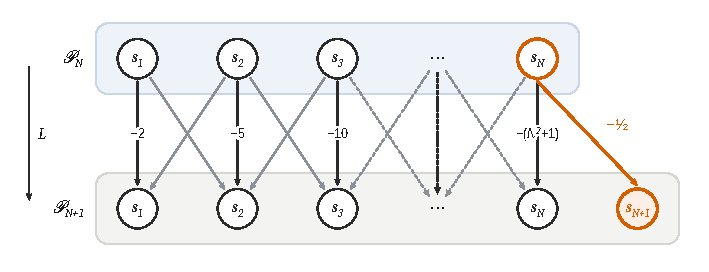
\includegraphics{figures/q18-action-l-base.pdf}
\caption*{Figure 1 --- Action de L sur la base des sₙ (coefficients −(n²+1) et
−1/2) : partant des N premiers vecteurs, seul le dernier atteint le
vecteur d'indice N+1}
\end{figure}

\emph{Injectivité.} Si \(p\neq0\), \(L(p)\) a une coordonnée non nulle, donc \(L(p)\neq0\). Ainsi \(\ker L=\{0\}\).

\emph{\(s_1\notin\operatorname{Im}L\).} Supposons \(s_1=L(p)\). Comme \(s_1\neq0=L(0)\), on a \(p\neq0\) ; soit \(N\) son plus haut indice.

La coordonnée de \(L(p)\) sur \(s_{N+1}\) est non nulle, alors que celle de \(s_1\) est nulle puisque \(N+1\ge2\). C'est contraire à l'unicité des coordonnées dans la base \((s_1,\dots,s_{N+1})\). Donc \(L\) n'est pas surjective.

\textbf{\(L\) est un endomorphisme injectif de \(\mathcal P\), et \(s_1\notin\operatorname{Im}L\).}

\begin{methode}

C'est l'argument du degré pour les polynômes : un opérateur qui augmente le degré d'exactement un est injectif. Ici \(\mathcal P\) est de dimension infinie, et \(L\) est injective sans être surjective, ce qui est impossible en dimension finie.

\end{methode}

\begin{jury}

Rapport 2026 : « La linéarité n'était pas le point essentiel. » Il fallait identifier le noyau et justifier la non-surjectivité par \(s_1\). Et « Peu de candidats ont pensé à montrer \(L(\mathcal P)\subset\mathcal P\) » : sans cette inclusion, \(L\) n'est pas un endomorphisme.

\end{jury}

\hypertarget{question-20}{%
\subsection{Question 20}\label{question-20}}

\begin{indication}{1}

Trois points : inclusion de la somme dans \(\mathcal P_{N+1}\), caractère direct, égalité des dimensions.

\end{indication}

\begin{indication}{2}

Pour le caractère direct, un élément de l'intersection s'écrit \(L(p)=\lambda s_1\) : utiliser Q19.

\end{indication}

\hypertarget{solution-19}{%
\subsubsection{Solution}\label{solution-19}}

Soit \(N\ge1\).

\emph{Inclusion.} Pour \(k\le N\), \(L(s_k)\in\mathcal P_{k+1}\subset\mathcal P_{N+1}\), donc \(L(\mathcal P_N)\subset\mathcal P_{N+1}\) ; et \(\mathcal P_1\subset\mathcal P_{N+1}\).

\emph{Somme directe.} Soit \(y\in L(\mathcal P_N)\cap\mathcal P_1\) : \(y=L(p)=\lambda s_1\) avec \(p\in\mathcal P_N\).

Si \(\lambda\neq0\), \(s_1=L(p/\lambda)\in\operatorname{Im}L\), ce qui contredit la question 19. Donc \(\lambda=0\) et \(y=0\).

\emph{Dimensions.} \(L\) est injective, donc \(\dim L(\mathcal P_N)=\dim\mathcal P_N=N\) (question 17), et
\equationajustee{\dim\big(L(\mathcal P_N)\oplus\mathcal P_1\big)=N+1.}
C'est la dimension de \(\mathcal P_{N+1}\). Un sous-espace d'un espace de dimension finie, de même dimension que lui, lui est égal :
\equationajustee{\boxed{\forall N\ge1,\quad L(\mathcal P_N)\oplus\mathcal P_1=\mathcal P_{N+1}.}}

\begin{piege}

Le comptage des dimensions ne suffit pas seul : il faut d'abord l'inclusion dans \(\mathcal P_{N+1}\), sans quoi on compare des espaces sans lien.

\end{piege}

\begin{jury}

Rapport 2026 : « Il s'agissait essentiellement de constater que l'image de \(\mathcal P_N\) par \(L\) était contenue dans \(\mathcal P_{N+1}\) ce qui n'a été que très rarement justifié. »

\end{jury}

\hypertarget{question-21}{%
\subsection{Question 21}\label{question-21}}

\begin{indication}{1}

Placer \(c\) dans un \(\mathcal P_{N+1}\) et le décomposer grâce à Q20.

\end{indication}

\begin{indication}{2}

La partie \(L(p)\) a un antécédent évident ; pour la partie \(\lambda s_1\), penser à la fonction \(g\) de Q16. Ne pas oublier de justifier la périodicité.

\end{indication}

\hypertarget{solution-20}{%
\subsubsection{Solution}\label{solution-20}}

Soit \(c\in\mathcal P\) : il existe \(N\ge1\) tel que \(c\in\mathcal P_N\subset\mathcal P_{N+1}\). Par la question 20, il existe \(p\in\mathcal P_N\) et \(\lambda\in\mathbb R\) tels que \(c=L(p)+\lambda s_1\).

Posons \(f=p+\lambda g\), où \(g\) est la fonction de la question 16. Alors \(f\) est de classe \(\mathcal C^2\) et, pour tout \(x\),
\equationajustee{\begin{aligned}
f''(x)-(1+\cos x)f(x)&=\underbrace{p''(x)-(1+\cos x)p(x)}_{L(p)(x)}+\lambda\underbrace{\big(g''(x)-(1+\cos x)g(x)\big)}_{\sin x}\\
&=c(x).
\end{aligned}}
Donc \(f\in\mathcal S(E)\).

\emph{Périodicité.} \(p\) est une combinaison finie de fonctions \(2\pi\)-périodiques.

Pour \(g\) : chaque somme partielle \(g_K:x\mapsto\sum_{n=1}^{K}a_n\sin(nx)\) est \(2\pi\)-périodique, et l'égalité \(g_K(x+2\pi)=g_K(x)\) passe à la limite \(K\to+\infty\) (séries convergentes).

\textbf{\(f=p+\lambda g\) est une solution \(2\pi\)-périodique de \((E)\).}

\begin{methode}

Par la partie 3, cette solution, bornée car continue et périodique, est l'unique solution bornée de \((E)\). Les parties 3 et 4 se complètent : unicité d'un côté, existence de l'autre.

\end{methode}

\hypertarget{partie-5-un-thuxe9oruxe8me-guxe9nuxe9ral}{%
\section{Partie 5 --- Un théorème général}\label{partie-5-un-thuxe9oruxe8me-guxe9nuxe9ral}}

On revient à \(b,c\) quelconques (\(c\neq0\)), en supposant l'existence d'une solution \(f_0\) bornée à dérivée bornée. Stratégie : tout se passe dans un espace de dimension finie (Q22), où une fonction continue atteint sa borne inférieure sur un fermé borné (Q23). Des moyennes de translatées de \(f_0\) montrent que cette borne est nulle (Q24), et le critère de Q4 conclut (Q25).

Le rapport 2026 qualifie cette partie de « partie peu abordée, du moins correctement » : c'est là que se font les écarts entre bonnes copies.

\hypertarget{question-22}{%
\subsection{Question 22}\label{question-22}}

\begin{indication}{1}

Par Q2, \(\mathcal B(E)\) s'écrit \(f_0+\mathcal B(H)\). Quel sous-espace vectoriel de dimension finie, formé de fonctions bornées, contient tous ces éléments ?

\end{indication}

\begin{indication}{2}

La dimension de \(\mathcal S(H)\) est majorée grâce au lemme d'unicité de Q4. Pour la fermeture, utiliser la caractérisation séquentielle et la continuité des formes linéaires en dimension finie.

\end{indication}

\begin{indication}{3}

Pour passer à la limite dans l'équation, fixer \(x\) et considérer la forme linéaire \(h\mapsto h''(x)+b(x)h(x)\) sur l'espace choisi.

\end{indication}

\hypertarget{solution-21}{%
\subsubsection{Solution}\label{solution-21}}

\emph{Choix de \(\mathcal H\).} Posons
\equationajustee{\boxed{\mathcal H=\mathbb Rf_0\oplus\mathcal B(H).}}
La somme est directe : si \(\lambda f_0\in\mathcal B(H)\) avec \(\lambda\neq0\), alors \(f_0\in\mathcal S(H)\), d'où \(c=f_0''+bf_0=0\), ce qui est exclu.

\(f_0\) est bornée, et \(\mathcal B(H)\) est un sous-espace vectoriel formé de fonctions bornées (question 1) : \(\mathcal H\) est un sous-espace vectoriel de \(\mathbf B(\mathbb R,\mathbb R)\).

Comme \(\mathcal B(H)\subset\mathcal S(H)\) et \(\dim\mathcal S(H)\le2\) (Q4), on a \(\dim\mathcal H\le3\).

Puisque \(f_0\in\mathcal B(E)\), la question 2 donne
\equationajustee{\mathcal A\subset\mathcal B(E)=f_0+\mathcal B(H)\subset\mathcal H.}
Les éléments de \(\mathcal H\) sont de classe \(\mathcal C^2\) (\(f_0\) et les solutions de \((EH)\) le sont). On munit \(\mathcal H\) de la norme \(\|\cdot\|\).

\emph{Non vide.} \(f_0\in\mathcal B(E)\) et \(\|f_0\|=M_0\) : \(f_0\in\mathcal A\).

\emph{Bornée.} \(\mathcal A\) est incluse dans la boule fermée de centre \(0\) et de rayon \(M_0\).

\emph{Fermée.} Soit \((f_n)\) une suite d'éléments de \(\mathcal A\) qui converge vers \(f\in\mathcal H\).

Pour \(x\in\mathbb R\) fixé, \(\ell_x:h\mapsto h''(x)+b(x)h(x)\) est une forme linéaire sur \(\mathcal H\), continue puisque \(\mathcal H\) est de dimension finie. Donc
\equationajustee{\ell_x(f)=\lim_{n\to+\infty}\ell_x(f_n)=c(x).}
Ceci pour tout \(x\) : \(f\in\mathcal S(E)\), et \(f\) est bornée (\(f\in\mathcal H\)), donc \(f\in\mathcal B(E)\). Enfin, pour tout \(n\),
\equationajustee{\begin{aligned}
\|f\|&\le\|f-f_n\|+\|f_n\|\\
&\le\|f-f_n\|+M_0.
\end{aligned}}
En faisant tendre \(n\) vers \(+\infty\), \(\|f\|\le M_0\). Donc \(f\in\mathcal A\) : \(\mathcal A\) est fermée dans \(\mathcal H\).

\textbf{\(\mathcal A\) est une partie fermée, bornée et non vide de \(\mathcal H\), de dimension finie (au plus 3).}

\begin{piege}

\(\mathcal A\) n'est \textbf{pas} la boule fermée de centre \(0\) et de rayon \(M_0\) : c'est son intersection avec \(\mathcal B(E)\). La fermeture de la boule ne suffit donc pas ; il faut aussi que la limite reste solution de \((E)\).

Pour \(\mathcal H\), l'espace \(\mathcal S(H)\) ne convient pas (ses éléments ne sont pas tous bornés), ni \(\mathcal B(E)\), qui n'est pas un sous-espace vectoriel (il ne contient pas \(0\), car \(c\neq0\)).

\end{piege}

\begin{jury}

Rapport 2026 : seuls quelques rares candidats ont proposé \(\mathcal H=\mathbb Rf_0\oplus\mathcal B(H)\), et « Un certain nombre de candidats confondent \(\mathcal A\) avec la boule fermée de centre 0 et de rayon \(M_0\) », ce qui rend fausse leur preuve de la fermeture.

\end{jury}

\begin{methode}

En dimension finie, toute forme linéaire est continue, même une forme qui fait intervenir des dérivées. C'est ce qui permet de passer à la limite dans l'équation alors que la convergence uniforme ne contrôle pas \(f''\) en général.

\end{methode}

\hypertarget{question-23}{%
\subsection{Question 23}\label{question-23}}

\begin{indication}{1}

Existence de \(\alpha\) : propriété de la borne inférieure dans \(\mathbb R\).

\end{indication}

\begin{indication}{2}

Pour l'atteinte, écrire \(\mathcal I\) comme l'image de \(\mathcal A\) par une fonction \(\Phi\) définie sur \(\mathcal H\) et montrer que \(\Phi\) est continue ; quel théorème du cours s'applique alors sur un fermé borné en dimension finie ?

\end{indication}

\hypertarget{solution-22}{%
\subsubsection{Solution}\label{solution-22}}

Soit \(\Phi:\mathcal H\to\mathbb R\) définie par \(\Phi(f)=|f(2\pi)-f(0)|+|f'(2\pi)-f'(0)|\), bien définie car \(\mathcal H\subset\mathcal C^2\). On a \(\mathcal I=\Phi(\mathcal A)\).

\emph{Existence de \(\alpha\).} \(\mathcal A\) est non vide, donc \(\mathcal I\) aussi, et \(\mathcal I\subset\mathbb R_+\) est minorée par \(0\). Sa borne inférieure existe donc, et elle est positive.

\emph{Continuité de \(\Phi\).} Les applications \(f\mapsto f(0)\), \(f\mapsto f(2\pi)\), \(f\mapsto f'(0)\) et \(f\mapsto f'(2\pi)\) sont des formes linéaires sur \(\mathcal H\).

Comme \(\mathcal H\) est de dimension finie, elles sont continues. Par différence, valeur absolue et somme, \(\Phi\) est continue sur \(\mathcal H\).

\emph{Atteinte.} Théorème des bornes atteintes : une fonction réelle continue sur une partie non vide, fermée et bornée d'un espace vectoriel normé de dimension finie est bornée et atteint ses bornes.

Il s'applique à \(\Phi\) sur \(\mathcal A\) (question 22) : il existe \(f_1\in\mathcal A\) tel que \(\Phi(f_1)=\inf_{\mathcal A}\Phi=\alpha\), soit
\equationajustee{\boxed{\alpha=|f_1(2\pi)-f_1(0)|+|f_1'(2\pi)-f_1'(0)|,\ f_1\in\mathcal A.}}

\begin{piege}

Invoquer la continuité de \(f\) et de \(f'\) : elle ne dit rien de la continuité de \(\Phi\), qui est une fonction \textbf{de la fonction} \(f\). Et la continuité de \(f\mapsto f'(2\pi)\) pour la norme infinie est fausse sur un espace de fonctions quelconque : elle ne tient que parce que \(\mathcal H\) est de dimension finie. C'est toute la raison d'être de la question 22.

\end{piege}

\begin{jury}

Rapport 2026 : la plupart citent la continuité de \(f\) et de \(f'\), « ce qui n'est évidemment pas le bon argument. Il fallait rappeler, qu'en dimension finie, l'application définissant l'ensemble \(\mathcal I\) était continue. » Séparer aussi l'existence de la borne inférieure (partie de \(\mathbb R\) non vide minorée) de son atteinte (théorème des bornes atteintes, hypothèses citées).

\end{jury}

\hypertarget{question-24}{%
\subsection{Question 24}\label{question-24}}

\begin{indication}{1}

Montrer que \(g_n\in\mathcal A\) : les \(T^k(f_0)\) sont des solutions de même norme que \(f_0\), et la moyenne a des coefficients de somme \(1\).

\end{indication}

\begin{indication}{2}

Dans \(g_n(2\pi)-g_n(0)\), écrire chaque terme \(T^k(f_0)(2\pi)\) en fonction de \(f_0\) : la somme télescope.

\end{indication}

\hypertarget{solution-23}{%
\subsubsection{Solution}\label{solution-23}}

\emph{\(g_n\in\mathcal A\).} Par récurrence sur \(k\) à l'aide de la question 3, \(T^k(f_0)\in\mathcal S(E)\) pour tout \(k\in\mathbb N\), et \(\|T^k(f_0)\|=\sup_x|f_0(x+2k\pi)|=M_0\).

Alors \(g_n\) est de classe \(\mathcal C^2\) et
\equationajustee{\begin{aligned}
g_n''+bg_n&=\frac1{n+1}\sum_{k=0}^n\big((T^kf_0)''+bT^kf_0\big)\\
&=\frac{1}{n+1}\sum_{k=0}^nc\\
&=c,
\end{aligned}}
donc \(g_n\in\mathcal S(E)\). De plus \(\|g_n\|\le\frac1{n+1}\sum_{k=0}^n\|T^k(f_0)\|=M_0\). Ainsi \(g_n\in\mathcal B(E)\) et \(\|g_n\|\le M_0\) : \(g_n\in\mathcal A\).

\emph{Télescopage.} On a \(T^k(f_0)(2\pi)=f_0(2(k+1)\pi)\) et \(T^k(f_0)(0)=f_0(2k\pi)\), donc
\equationajustee{\begin{aligned}
g_n(2\pi)-g_n(0)&=\frac1{n+1}\sum_{k=0}^n\big(f_0(2(k+1)\pi)-f_0(2k\pi)\big)\\
&=\frac{f_0(2(n+1)\pi)-f_0(0)}{n+1},
\end{aligned}}
de valeur absolue au plus \(\frac{2M_0}{n+1}\). De même \(g_n'(x)=\frac1{n+1}\sum_{k=0}^nf_0'(x+2k\pi)\), et
\equationajustee{\begin{aligned}
|g_n'(2\pi)-g_n'(0)|&=\frac{|f_0'(2(n+1)\pi)-f_0'(0)|}{n+1}\\
&\le\frac{2M_1}{n+1}.
\end{aligned}}

\emph{Conclusion.} \(g_n\in\mathcal A\), donc \(\Phi(g_n)\in\mathcal I\) et
\equationajustee{\boxed{\begin{aligned}
\forall n\in\mathbb N,\quad\alpha&\le\Phi(g_n)\\
&\le\frac{2(M_0+M_1)}{n+1}.
\end{aligned}}}

\begin{piege}

Sans le facteur \(\frac1{n+1}\), la somme \(\sum_kT^k(f_0)\) serait solution de \(y''+by=(n+1)c\), et non de l'équation étudiée. Une combinaison de solutions de \((E)\) est solution de \((E)\) si et seulement si ses coefficients ont pour somme \(1\).

\end{piege}

\begin{methode}

Moyennes de Cesàro de translatées : la moyenne de \(n+1\) translatées successives « presque » recolle, avec un défaut qui décroît en \(1/(n+1)\) grâce au télescopage. C'est l'idée des théorèmes ergodiques élémentaires.

\end{methode}

\begin{jury}

Rapport 2026 : « La question n'a pratiquement jamais été abordée correctement. » Les deux points à rédiger sont l'appartenance \(g_n\in\mathcal A\) (solution, bornée, norme au plus \(M_0\)) et le télescopage.

\end{jury}

\hypertarget{question-25}{%
\subsection{Question 25}\label{question-25}}

\begin{indication}{1}

Faire tendre \(n\) vers l'infini dans Q24 pour obtenir la valeur de \(\alpha\).

\end{indication}

\begin{indication}{2}

Utiliser ensuite la fonction \(f_1\) de Q23, qui réalise \(\alpha\), et le critère de la partie 1.

\end{indication}

\hypertarget{solution-24}{%
\subsubsection{Solution}\label{solution-24}}

Par les questions 23 et 24, \(0\le\alpha\le\frac{2(M_0+M_1)}{n+1}\) pour tout \(n\in\mathbb N\). Le majorant tend vers \(0\), donc \(\alpha=0\).

La fonction \(f_1\in\mathcal A\) de la question 23 vérifie donc
\equationajustee{|f_1(2\pi)-f_1(0)|+|f_1'(2\pi)-f_1'(0)|=0.}
Une somme de deux réels positifs est nulle : \(f_1(2\pi)=f_1(0)\) et \(f_1'(2\pi)=f_1'(0)\).

Comme \(f_1\in\mathcal A\subset\mathcal B(E)\subset\mathcal S(E)\), la question 4 s'applique : \(f_1\) est \(2\pi\)-périodique.

\textbf{\((E)\) possède une solution \(2\pi\)-périodique, à savoir \(f_1\) : le théorème est démontré.}

\begin{piege}

On ne peut pas « passer à la limite » sur les \(g_n\) : rien ne dit qu'elles convergent. C'est précisément pour éviter ce problème que le sujet passe par l'atteinte de la borne inférieure : \(\alpha=0\) ne servirait à rien si \(\alpha\) n'était pas un minimum.

\end{piege}

\begin{jury}

Rapport 2026 : « Question simple traitée par quelques candidats. » Elle se rédige en admettant Q23 et Q24 : c'est une question à ne pas laisser de côté.

\end{jury}

\begin{methode}

Schéma d'existence par minimisation : définir une fonction « défaut » continue, minorée par \(0\), sur un compact (fermé borné en dimension finie) ; montrer que son infimum vaut \(0\) ; un point où le minimum est atteint est un point où le défaut s'annule.

\end{methode}

\hypertarget{bilan}{%
\section{Bilan}\label{bilan}}

\textbf{Méthodes à retenir.}

\begin{itemize}
\tightlist
\item
  \emph{Unicité par l'énergie} : une solution de \(y''+by=0\) nulle en un point avec sa dérivée est nulle (Q4), par l'étude de \(h^2+h'^2\), sans le théorème de Cauchy, hors programme de PC à cet ordre. Avec la translation \(T\), c'est le critère de périodicité « recollement en valeur et en pente ».
\item
  \emph{Raisonner sur l'équation plutôt que sur la forme des solutions} (Q7) : la périodicité de \(f\) se transmet à \(f''+\omega^2f\), donc au second membre.
\item
  \emph{Déterminant non nul, système de Cramer} (Q9) : à énoncer dans le bon sens.
\item
  \emph{Unicité + invariance donne la symétrie} (Q14) : la solution bornée unique est fixée par \(T\).
\item
  \emph{Convexité par la dérivée seconde} et calcul patient de \((g^2)''\) avec le terme \(2g'^2\) (Q11--Q12) ; de \(g^2\) constante à \(g\) constante par continuité.
\item
  \emph{Amélioration itérée d'une majoration} par une relation de récurrence (Q15) ; \emph{dérivation terme à terme} sous convergence normale des séries dérivées, théorème énoncé (Q16).
\item
  \emph{Linéarisation et réindexation} de produits \(\cos x\sin(nx)\) (Q16, Q18).
\item
  \emph{Argument de degré} pour un opérateur qui augmente l'indice maximal de un : stabilité de \(\mathcal P\), injectivité, non-surjectivité, supplémentaire de l'image (Q19--Q20).
\item
  \emph{Dimension finie} : continuité automatique des formes linéaires (même faisant intervenir des dérivées), caractérisation séquentielle des fermés, théorème des bornes atteintes (Q22--Q23).
\item
  \emph{Moyennes de translatées et télescopage} (Q24), puis \emph{existence par minimisation} (Q25).
\end{itemize}

\textbf{Questions discriminantes.} D'après le rapport 2026, les points se sont joués sur le caractère borné (Q1, Q2), la dérivée seconde de \(g^2\) (Q11), la continuité de \(g\) (Q12), Q14, la série \(\sum n^2a_n\) (Q15), la dérivation terme à terme (Q16), les inclusions de Q19--Q20, et toute la partie 5, peu ou mal abordée. Q4 a été neutralisée.

\textbf{Prérequis à revoir.} Principe de superposition ; équations à coefficients constants ; séries de Riemann et comparaison ; théorème de dérivation des séries de fonctions (classe \(\mathcal C^k\)) ; formules de linéarisation ; bases, dimension, somme directe ; topologie des espaces vectoriels normés de dimension finie.

\textbf{Questions transposables.} Le critère de Q4 vaut pour toute équation linéaire à coefficients périodiques. Le calcul de Q8--Q9 est le calcul type des solutions périodiques d'un oscillateur harmonique forcé : il y a des solutions périodiques autres que la solution forcée exactement quand les périodes propre et forcée sont commensurables.

L'argument de convexité de Q11--Q12 s'adapte à toute équation \(y''=q(x)y\) avec \(q\ge0\) non identiquement nulle. Le schéma de la partie 5 (dimension finie, minimisation d'un défaut, moyennes de Cesàro) est un classique des problèmes d'existence de solutions périodiques (théorème de Massera).

\end{document}
